\chapter{SOLUTION PROCEDURE}
\section{Calculate Kelp Density}
\subsection{Relative coordinate system}
\label{sec:rel_coords}
To determine under what conditions a frond will occupy a given point, we begin by
describing the shape of the frond in Cartesian and then converting to polar coordinates.
Of primary interest are the edges connected to the frond tip.
For convenience, we will use a relative coordinate system $(\theta',s)$ such that the line connecting the base to the tip is vertical, with the base at $(0,0)$.
The Cartesian analogue of this coordinate system, $(x',y')$, has the following properties.
\begin{align}
	x' &= s\cos\theta' \\ 
	y' &= s\sin\theta'
\end{align}
and
\begin{align}
	s &= \sqrt{x'^2+y'^2}
\end{align}
\vspace{-1em}
\begin{align}
	\theta' &= \atantwo(y, x)
\end{align}

\subsection{Functional description of frond edge}
With this coordinate system established, we can describe the outer two edges of the frond in Cartesian coordinates as a piecewise linear function connecting the left corner: $(-w/2,f_a)$, the tip: $(0,l)$, and the right corner: $(w/2,f_a)$.
This function has the form
\begin{equation}
	y'_f(x') = l-\sign(x')\frac{f_b}{w/2}x'.
\end{equation}

Using the equations in section \ref{sec:rel_coords}, this can be written in polar coordinates after some rearrangement as
\begin{equation}
	s_f'(\theta') = \frac{l}{\sin\theta' + S(\theta')\frac{2f_b}{w}\cos\theta'}
\end{equation}
where
\begin{equation}
	S(\theta') = \sign(\theta'-\pi/2)
\end{equation}

Then, using the relationships in section \ref{sec:shape}, we can rewrite the above equation in terms of our frond ratios $f_s$ and $f_r$.
\begin{equation}
	\label{eq:rf_rel}
	s_f'(\theta') = \frac{l}{\sin\theta' + S(\theta')\frac{2f_r}{1+f_s}\cos\theta'}
\end{equation}

\subsection{Absolute coordinates}
\label{sec:abs_coords}
To generalize to a frond pointed at an angle $\theta_f$, we will use the coordinate system $(\theta,s)$ such that
\begin{equation}
	\theta = \theta' + \theta_f - \frac{\pi}{2}
\end{equation}
Then, for a frond pointed at the arbitrary angle $\theta_f$, the function for the outer edges can be written as 
\begin{equation}
	\label{eq:rf_abs}
	s_f(\theta) = s_f'\left(\theta - \theta_f + \frac{\pi}{2} \right)
\end{equation}


\subsection{Conditions for occupancy}
Consider a fixed frond of length $l$ at an angle $\theta_f$. The point
$(\theta,s)$ is occupied by the frond if
\begin{align}
	\left|\theta_f - \theta \right| < \alpha
	\shortintertext{and}
	s < s_f(\theta)
\end{align}

Equivalently, letting the point $(\theta,s)$ be fixed, a frond occupies the point if the following conditions are satisfied.
\begin{align}
	\theta - \alpha < \theta_f < \theta + \alpha
	\label{eqn:rs_th}
	\shortintertext{and}
	l > l_{min}(\theta,s)
	\label{eqn:rs_l}
\end{align}
where
\begin{equation}
	l_{min}(\theta,s) = s \cdot \frac{l}{s_f(\theta)}
\end{equation}


Then, considering the point to be fixed, \eqref{eqn:rs_th} and \eqref{eqn:rs_l} define the spacial region $R_s(\theta,s)$ called the ``occupancy region for $(\theta,s)$'' with the property that if the tip of a frond lies within this region (i.e. $(\theta_f,l) \in R_s(\theta,s)$), then it occupies the point.
$R_s(3\pi/4,3/2)$ is shown in blue in figure \ref{fig:shade_area} and the smallest possible occupying fronds for several values of $\theta_f$ are shown in various colors.
Any frond longer than these at the same angle will also occupy the point.

\begin{figure}[h]
	\centering
	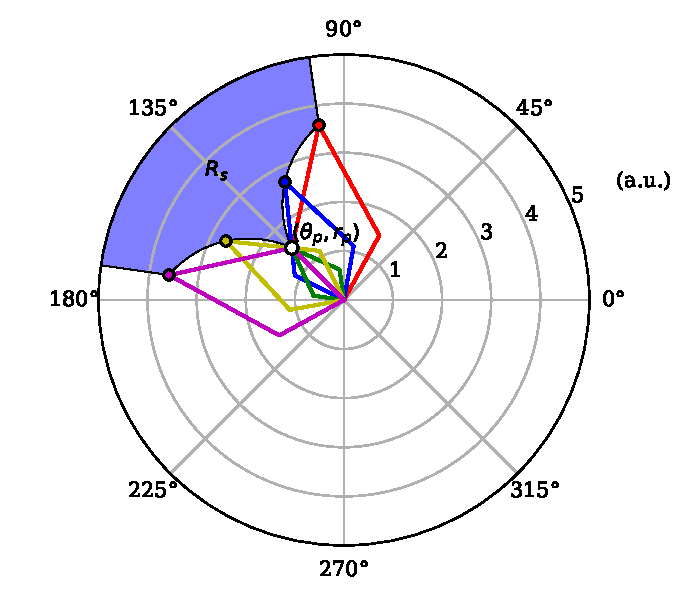
\includegraphics[width=.75\linewidth]{shade_area}
	\vspace{-2em}
	\captionof{figure}{Outlines of minimum-length fronds for a variety of angles to occupy the point $(\theta,s)=(3\pi/4,3/2)$}
	\label{fig:shade_area}
\end{figure}

\subsection{Probability of occupancy}
% TODO: Double check
We are interested in the probability that, given a fixed point $(\theta,s)$, values of $l$ and $\theta_f$ chosen from the distributions described in section \ref{sec:dist} will fall in the occupancy region.
This is found by integrating $P_{2D}$ over the occupancy region for $(\theta,s)$, as depicted in figure \ref{fig:cart_shade}.

\begin{figure}[h]
	\centering
	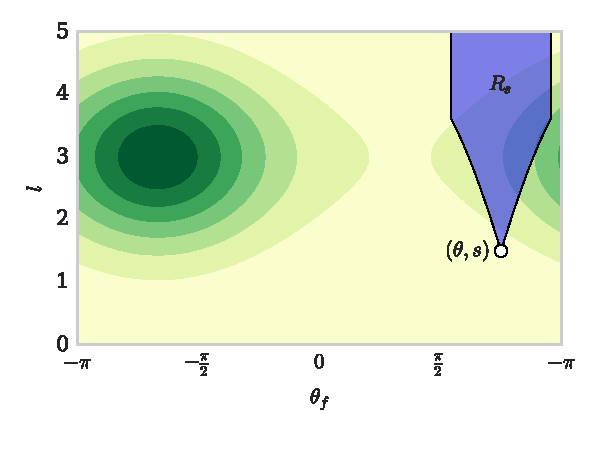
\includegraphics[width=.75\linewidth]{cart_shade}
	\vspace{-3em}
	\captionof{figure}{Contour plot of $P_{2D}(\theta_f,l)$ overlayed with the
    region in the $\theta_f-l$ plane which results in a frond occupying the point $(\theta,s)=(3\pi/4,3/2)$}
	\label{fig:cart_shade}
\end{figure}

Now, integrating $P_{2D}(\theta_f,l)$ over $R_s(\theta,s)$ yields the proportion of the population occupying the point $(\theta,s)$.
\begin{align}
		\tilde{P}_k(\theta,s,z)	&= \iint_{R_s(\theta,s)}
								P_{2D}(\theta_f,l)
								\,dl\,d\theta_f \nonumber \\
							&= \int_{\theta-\alpha}^{\theta+\alpha} 
								\int_{l_{min}(\theta_f)}^\infty
								P_{2D}(\theta_f,l)
								\,dl\,d\theta_f
\end{align}

% TODO: Revise. This is the first mention of grid cells.
Then, multiplying $\tilde{P}_k$ by the number of fronds in the population $n$ of the depth layer gives the expected number of fronds occupying the point.
Now, assuming a uniform thickness $t$ for all fronds, and a thickness $dz$ of the depth layer, we find the proportion of the grid cell occupied by kelp to be
\begin{equation}
  P_k = \frac{nt}{dz}\tilde{P}.
\end{equation}

Then, the effective absorption coefficien can be calculated at any point in space as
\begin{equation}
  a(\vec{x}) = P_k(\vec{x})a_k + (1-P_k(\vec{x}))a_w
\end{equation}
% TODO: Calculate absorption coefficient grid.

\begin{figure}[h]
	\centering
	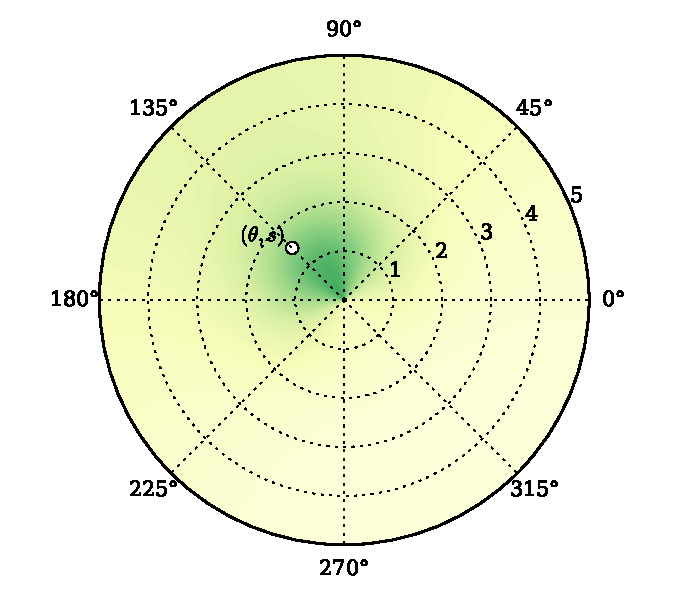
\includegraphics[width=.75\linewidth]{prob_shade}
	\vspace{-2em}
	\captionof{figure}{Contour plot of the probability of occupying sampled at 121 points using $\theta_f=2\pi/3,v_w=1$}
	\label{fig:prob_shade}
\end{figure}

\subsection{Absorbed Light}
% TODO: This.
** ADD WORDS

\newcommand{\abslight}{\mathcal{L}}
\begin{align}
  \abslight_{kq} &= \frac{dz_k}{t}
  \cdot \left(\frac{A_{kq}\mbox{ind}_{kq}}{\sum_{q'}A_{kq'}\mbox{ind}_{kq'}}\right)
  \cdot \frac{1}{\mbox{ind}_{kq}}
  \cdot \sum_{i=1}^{n_x}\sum_{j=1}^{n_y}P_{ijk}I_{ijk} \\
  &= \frac{dz_k A_{kq}}{t}
  \cdot \frac{\sum_{ij}P_{ijk}I_{ijk}}{\sum_{q'}A_{kq'}\mbox{ind}_{kq'}}
\end{align}


\section{Asymptotics}
\subsection{Substitute asymptotic series}
\newcommand{\Lasym}{L_0(\vec{x},\vec{\omega}) + b L_1(\vec{x},\vec{\omega}) + b^2 L_2(\vec{x},\vec{\omega}) + \cdots}
\newcommand{\Lasymp}{L_0(\vec{x},\vec{\omega}') + b L_1(\vec{x},\vec{\omega}') + b^2 L_2(\vec{x},\vec{\omega}') + \cdots}
\begin{align}
  L(\vec{x},\vec{\omega}) = \Lasym
\end{align}

Then, substituting the above into the RTE,

\begin{equation}
  \begin{split}
    &\vec{\omega} \cdot \nabla \left[ \Lasym \right] \\
    &+ a(\vec{x}) \left[ \Lasym \right] \\
    &= b\Bigg(
      \int_{4\pi} \beta(\abs{\vec{\omega} - \vec{\omega}'})
      \left[ \Lasymp \right] \, d\vec{\omega}' \\
    &- \left[ \Lasym \right]
    \Bigg)
    \end{split}
\end{equation}

Now, grouping like powers of $b$, we have the decoupled set of equations
\begin{align}
  \vec{\omega} \cdot \nabla L_0(\vec{x}, \vec{\omega}) + a(\vec{x})L_0(\vec{x}) &= 0 \\
  \vec{\omega} \cdot \nabla L_1(\vec{x}, \vec{\omega}) + a(\vec{x})L_1(\vec{x})
  &= \int_{4\pi} \beta(\abs{\vec{\omega} - \vec{\omega}'}) L_0(\vec{x}, \vec{\omega}')\,d\vec{\omega}' - L_0(\vec{x}, \vec{\omega}) \\ 
  \vec{\omega} \cdot \nabla L_2(\vec{x}, \vec{\omega}) + a(\vec{x})L_2(\vec{x})
  &= \int_{4\pi} \beta(\abs{\vec{\omega} - \vec{\omega}'}) L_1(\vec{x}, \vec{\omega}')\,d\vec{\omega}' - L_1(\vec{x}, \vec{\omega}) \\ 
  &\vdots \nonumber
\end{align}

\subsection{Boundary Conditions}

% TODO: Asymptotic boundary conditions
 
\subsection{Rewrite as ODE along ray path}
For all $\vec{x}, \vec{\omega}$, let
\begin{align}
  \tilde{a}(s) &= a(\vec{l}(\vec{x}, \vec{\omega}), s), \\ 
  \frac{du_0}{ds}(s) + \tilde{a}(s) u_0(s) &= 0, u_0(0) = f(\vec{\omega})
\end{align}
Then,
\begin{align}
  u_0(s) = f(\omega) \exp\left(-\int_0^s \tilde{a}(s)\, ds\right), \\
  L_0(\vec{l}(\vec{x}, \vec{\omega},s), \vec{\omega}) = u_0(s)
\end{align}

\begin{align}
  g_n(s) = \int_{4\pi} \beta(\abs{\vec{\omega} - \vec{\omega}'})
  L_{n-1}(\vec{l}(\vec{x}, \vec{\omega'}, s), \vec{\omega}')\,d\vec{\omega}' - L_{n-1}(\vec{l}(\vec{x}, \vec{\omega}, s), \vec{\omega}) \\ 
  \frac{du_n}{ds}(s) + \tilde{a}(s)u_n(s) = g_n(s), u_n(0) = 0
\end{align}

Then,
\begin{align}
  u_n(s) = \int_0^sg_n(s')\exp\left( -\int_{s''}^{s'}\tilde{a}(s'')\,ds'' \right)\, ds' \\
  L_n(\vec{l}(\vec{x}, \vec{\omega}, s), \vec{\omega}) = u_n(s)
\end{align}
